\documentclass[compress]{beamer}
\usetheme{Warsaw}
\usecolortheme{seagull}
\usefonttheme[onlylarge]{structurebold}
\setbeamerfont*{frametitle}{size=\normalsize,series=\bfseries}
\setbeamertemplate{navigation symbols}{}
\setbeamertemplate{footline}
{%
\begin{beamercolorbox}[wd=0.5\textwidth,ht=3ex,dp=1.5ex,leftskip=.5em,rightskip=.5em]{author
in head/foot}%
\usebeamerfont{author in head/foot}%
\hfill\insertshortauthor%
\end{beamercolorbox}%
\vspace*{-4.5ex}\hspace*{0.5\textwidth}%
\begin{beamercolorbox}[wd=0.5\textwidth,ht=3ex,dp=1.5ex,left,leftskip=.5em]{title
in head/foot}%
\usebeamerfont{title in head/foot}%
\insertshorttitle\hfill\insertframenumber/\inserttotalframenumber%
\end{beamercolorbox}%
}
\logo{
\includegraphics[height=0.5cm]{img/geany.png}}
\beamertemplatesolidbackgroundcolor{black!5}
\beamertemplatetransparentcovered
\usepackage[utf8]{inputenc}
\usepackage[german]{babel}
\usepackage{graphicx}
\title{Geany -- Just Not Another Editor \\ Eine kurze Einführung in Geany}
\author{Frank Lanitz \\ frank@frank.uvena.de}
\date{20.10.2011}
\usepackage{listings,color}
\usepackage{courier}
\usepackage{tikz}
\lstset{basicstyle=\ttfamily\scriptsize}
\lstset{showspaces=false}
\lstset{showtabs=false}
\lstset{showstringspaces=false}
\lstset{keywordstyle=\bfseries}
\lstset{tabsize=4}
\lstset{frameround=ffff}
\lstset{extendedchars=true}
\lstset{stringstyle=\ttfamily}
\lstset{commentstyle=\ttfamily}
\lstset{captionpos=b}

% Einkommentieren und über Positivliste die gewollten
% Teile aktivieren.
%\includeonly{}
\begin{document}
\frame{\titlepage}
\frame{\tableofcontents}
\begin{frame}
	\frametitle{Kurzvorstellung}
	\begin{block}{Über mich}
		\begin{itemize}
			\item Systembetreuer an der Universität Jena 
				\begin{itemize}
					\item Linux
					\item PostgreSQL
					\item ...
				\end{itemize}
			\item Im Vorstand des Hackspace Jena e.V.
			\item Aktiv im Umfeld der FLOSS
			\item Mitarbeit bei Geany seit ca. 6 Jahren u.a. 
			\begin{itemize}
				\item Übersetzungen
				\item Maintainer verschiedener Plugins
				\item Mailingliste, IRC, \dots
			\end{itemize}
		\end{itemize}
	\end{block}
\end{frame}
\section[Einordnung]{Einordnung von Geany}
\begin{frame}
	\frametitle{Geany in die Welt von Anjuta, emacs, vim \& co}
	\begin{block}{Was ist Geany?}
		\begin{itemize}
			\item Entwicklungsumgebung
			\item Entwicklung seit 2005
			\item Aktuelle Version 0.18.1 vom 14. Februar 2010
			\item Ziel: Geringe Systemanforderungen und wenige
				  Abhängigkeiten zu anderen Paketen
			\item Realisiert in C mit Teilen in C++
			\item Basierend auf Scintilla und GTK2 ($>=$ 2.8)
			\item Lizenz: GPLv2+
		\end{itemize}
	\end{block}
\end{frame}

\begin{frame}
	\frametitle{Einordnung von Geany in die Welt von Anjuta, emacs, vim \& co}
	\begin{figure}[ht]
		\centering
 		\footnotesize
		% Graphic for TeX using PGF
% Title: /home/frank/Diagramm1.dia
% Creator: Dia v0.96.1
% CreationDate: Mon Mar  9 21:37:47 2009
% For: frank
% \usepackage{tikz}
% The following commands are not supported in PSTricks at present
% We define them conditionally, so when they are implemented,
% this pgf file will use them.
\ifx\du\undefined
  \newlength{\du}
\fi
\setlength{\du}{15\unitlength}
\begin{tikzpicture}
\pgftransformxscale{1.000000}
\pgftransformyscale{-1.000000}
\definecolor{dialinecolor}{rgb}{0.000000, 0.000000, 0.000000}
\pgfsetstrokecolor{dialinecolor}
\definecolor{dialinecolor}{rgb}{1.000000, 1.000000, 1.000000}
\pgfsetfillcolor{dialinecolor}
\definecolor{dialinecolor}{rgb}{1.000000, 1.000000, 1.000000}
\pgfsetfillcolor{dialinecolor}
\pgfpathellipse{\pgfpoint{5.858894\du}{22.094996\du}}{\pgfpoint{2.423416\du}{0\du}}{\pgfpoint{0\du}{1.570716\du}}
\pgfusepath{fill}
\pgfsetlinewidth{0.050000\du}
\pgfsetdash{}{0pt}
\pgfsetdash{}{0pt}
\definecolor{dialinecolor}{rgb}{0.000000, 0.000000, 0.000000}
\pgfsetstrokecolor{dialinecolor}
\pgfpathellipse{\pgfpoint{5.858894\du}{22.094996\du}}{\pgfpoint{2.423416\du}{0\du}}{\pgfpoint{0\du}{1.570716\du}}
\pgfusepath{stroke}
\definecolor{dialinecolor}{rgb}{1.000000, 1.000000, 1.000000}
\pgfsetfillcolor{dialinecolor}
\pgfpathellipse{\pgfpoint{15.115650\du}{16.114764\du}}{\pgfpoint{3.275061\du}{0\du}}{\pgfpoint{0\du}{1.749584\du}}
\pgfusepath{fill}
\pgfsetlinewidth{0.050000\du}
\pgfsetdash{}{0pt}
\pgfsetdash{}{0pt}
\definecolor{dialinecolor}{rgb}{0.000000, 0.000000, 0.000000}
\pgfsetstrokecolor{dialinecolor}
\pgfpathellipse{\pgfpoint{15.115650\du}{16.114764\du}}{\pgfpoint{3.275061\du}{0\du}}{\pgfpoint{0\du}{1.749584\du}}
\pgfusepath{stroke}
\definecolor{dialinecolor}{rgb}{1.000000, 0.647059, 0.000000}
\pgfsetfillcolor{dialinecolor}
\pgfpathellipse{\pgfpoint{9.972793\du}{19.076297\du}}{\pgfpoint{3.177806\du}{0\du}}{\pgfpoint{0\du}{1.478041\du}}
\pgfusepath{fill}
\pgfsetlinewidth{0.050000\du}
\pgfsetdash{}{0pt}
\pgfsetdash{}{0pt}
\definecolor{dialinecolor}{rgb}{0.000000, 0.000000, 0.000000}
\pgfsetstrokecolor{dialinecolor}
\pgfpathellipse{\pgfpoint{9.972793\du}{19.076297\du}}{\pgfpoint{3.177806\du}{0\du}}{\pgfpoint{0\du}{1.478041\du}}
\pgfusepath{stroke}
\definecolor{dialinecolor}{rgb}{1.000000, 1.000000, 1.000000}
\pgfsetfillcolor{dialinecolor}
\pgfpathellipse{\pgfpoint{16.276869\du}{21.396201\du}}{\pgfpoint{2.889298\du}{0\du}}{\pgfpoint{0\du}{1.504087\du}}
\pgfusepath{fill}
\pgfsetlinewidth{0.050000\du}
\pgfsetdash{}{0pt}
\pgfsetdash{}{0pt}
\definecolor{dialinecolor}{rgb}{0.000000, 0.000000, 0.000000}
\pgfsetstrokecolor{dialinecolor}
\pgfpathellipse{\pgfpoint{16.276869\du}{21.396201\du}}{\pgfpoint{2.889298\du}{0\du}}{\pgfpoint{0\du}{1.504087\du}}
\pgfusepath{stroke}
\pgfsetlinewidth{0.100000\du}
\pgfsetdash{}{0pt}
\pgfsetdash{}{0pt}
\pgfsetbuttcap
{
\definecolor{dialinecolor}{rgb}{0.000000, 0.000000, 0.000000}
\pgfsetfillcolor{dialinecolor}
% was here!!!
\pgfsetarrowsend{stealth}
\definecolor{dialinecolor}{rgb}{0.000000, 0.000000, 0.000000}
\pgfsetstrokecolor{dialinecolor}
\draw (2.519705\du,24.037314\du)--(21.791725\du,24.037314\du);
}
\pgfsetlinewidth{0.100000\du}
\pgfsetdash{}{0pt}
\pgfsetdash{}{0pt}
\pgfsetbuttcap
{
\definecolor{dialinecolor}{rgb}{0.000000, 0.000000, 0.000000}
\pgfsetfillcolor{dialinecolor}
% was here!!!
\pgfsetarrowsend{stealth}
\definecolor{dialinecolor}{rgb}{0.000000, 0.000000, 0.000000}
\pgfsetstrokecolor{dialinecolor}
\draw (2.989313\du,24.434675\du)--(2.986247\du,12.568023\du);
}
% setfont left to latex
\definecolor{dialinecolor}{rgb}{0.000000, 0.000000, 0.000000}
\pgfsetstrokecolor{dialinecolor}
\node[anchor=west] at (8.979390\du,19.256916\du){Geany};
% setfont left to latex
\definecolor{dialinecolor}{rgb}{0.000000, 0.000000, 0.000000}
\pgfsetstrokecolor{dialinecolor}
\node[anchor=west] at (4.973862\du,22.275614\du){nano};
% setfont left to latex
\definecolor{dialinecolor}{rgb}{0.000000, 0.000000, 0.000000}
\pgfsetstrokecolor{dialinecolor}
\node[anchor=west] at (14.434558\du,21.649068\du){vim, emacs};
% setfont left to latex
\definecolor{dialinecolor}{rgb}{0.000000, 0.000000, 0.000000}
\pgfsetstrokecolor{dialinecolor}
\node[anchor=west] at (12.912101\du,15.753526\du){Anjuta, Eclipse };
% setfont left to latex
\definecolor{dialinecolor}{rgb}{0.000000, 0.000000, 0.000000}
\pgfsetstrokecolor{dialinecolor}
\node[anchor=west] at (12.912101\du,16.553526\du){Visual Studio };
% setfont left to latex
\definecolor{dialinecolor}{rgb}{0.000000, 0.000000, 0.000000}
\pgfsetstrokecolor{dialinecolor}
\node[anchor=west] at (8.787175\du,24.850099\du){Lernaufwand \& Möglichkeiten};
% setfont left to latex
\definecolor{dialinecolor}{rgb}{0.000000, 0.000000, 0.000000}
\pgfsetstrokecolor{dialinecolor}
\node[anchor=west] at (4.651006\du,13.055694\du){};
% setfont left to latex
\definecolor{dialinecolor}{rgb}{0.000000, 0.000000, 0.000000}
\pgfsetstrokecolor{dialinecolor}
\node[anchor=west] at (3.169932\du,14.428397\du){System-};
% setfont left to latex
\definecolor{dialinecolor}{rgb}{0.000000, 0.000000, 0.000000}
\pgfsetstrokecolor{dialinecolor}
\node[anchor=west] at (3.169932\du,15.228397\du){anforderungen};
\end{tikzpicture}

	\end{figure}
\end{frame}

\begin{frame}
	\begin{figure}
		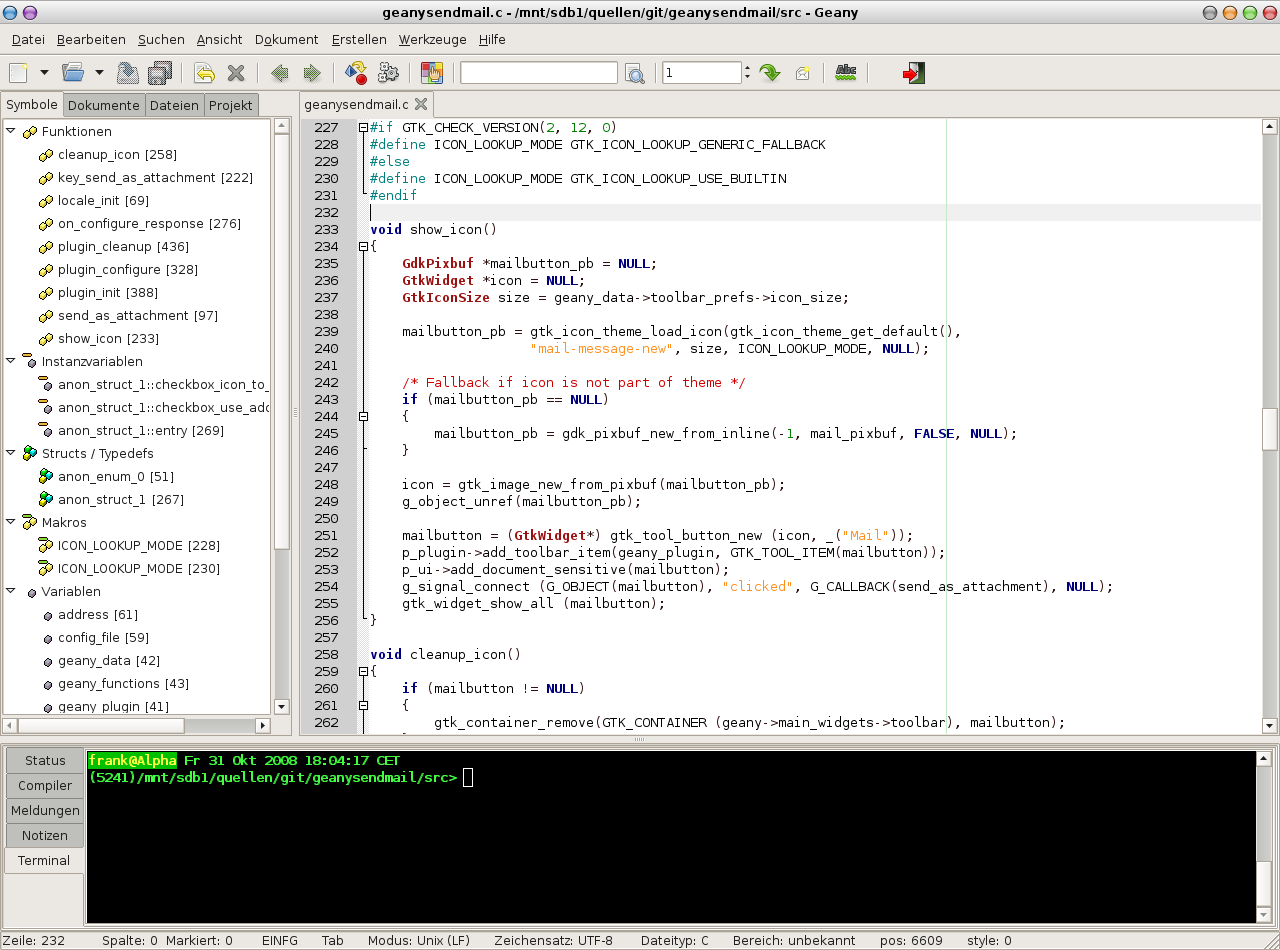
\includegraphics[scale=0.3]{../img/C_mit_symbol_2.png}\\
		\tiny C in Geany
	\end{figure}
\end{frame}

\section{Features}
\begin{frame}[allowframebreak]
	\frametitle{Features von Geany}
	\begin{block}{Visualisierung}
		\begin{itemize}
			\item Syntaxhervorherbung für verschiedenste Dateitypen $>$30
			\item Markierung von Fehlern beim Übersetzen
		\end{itemize}
	\end{block}
	\begin{block}{Entwicklung}
		\begin{itemize}
			\item Anpassbares Erstellen-Menü
			\item Plugins für Debugging, Versionskontrolle etc.
		\end{itemize}
	\end{block}
	\begin{block}{Unterstützung}
		\begin{itemize}
			\item Autovervollständigung von bekannten Symbolen,
				  Variablen, Markos etc.
			\item Templates
			\item Einfaches Einfügen von Quellcodeschnipseln
		\end{itemize}
	\end{block}
\end{frame}
\begin{frame}[allowframebreak]
	\frametitle{Features von Geany}
	\begin{block}{Navigation}
		\begin{itemize}
			\item Symbolbrowser zum einfachen Navigieren innerhalb
			      eines Dokumentes
			\item Funktion zum Springen zur Definition/Deklaration
			      einer Funktion
			\item Öffnen einer verlinkten Datei über das Kontextmenü
		\end{itemize}
	\end{block}
	\begin{block}{Sonstiges}
		\begin{itemize}
			\item Plattformunabhängig: (Linux, Unix, Windows)
			\item Erweiterbar: Pluginschnittstelle
			\item und noch ein paar mehr ...
		\end{itemize}
	\end{block}
\end{frame}

%\begin{frame}
	\frametitle{Codeschnipsel}
	\begin{block}{}
		\begin{itemize}
			\item Einfaches Definieren über Key-Value-Konfigurationsdatei
				  \texttt{snippets.conf}
			\item Aufruf über Schlagwort + Tastenkombination (frei wählbar)
			\item Dateitypspezifische Ersetzungen möglich
			\item Platzhalter zusätzlich für
				\begin{itemize}
					\item Neupositionierung des Cursors (auch mehrmals)
					\item Einrückungen basierend auf aktuellen Einstellungen
						  werden übernommen
				\end{itemize}
			\item Verschachtelung möglich
			\item Lokal und global definierbar; lokale Einstellung
				  ergänzt bzw. überschreibt globale Einstellung
		\end{itemize}
	\end{block}
\end{frame}

\begin{frame}[containsverbatim]
	\frametitle{Codeschnipsel Beispiele I}
	\begin{block}{Beispiel für C++}
		\begin{figure}[!h]
			\begin{lstlisting}[frame=none]
[Special]
brace_open=\n{\n\t
brace_close=}\n
block=\n{\n\t%cursor%\n}
block_cursor=\n{\n\t%cursor%\n}\n%cursor%

[C++]
for=for (int i = 0; i < %cursor%; i++)%brace_open%\n%brace_close%
			\end{lstlisting}
		\end{figure}
	\end{block}

	\begin{block}{Ergibt}
		\begin{figure}[!h]
			\begin{lstlisting}[frame=none, language=C++]
for (int i = 0; i < %csr%;; i++)
{
	%csr%;
}
%csr%;
			\end{lstlisting}
		\end{figure}
	\end{block}
\end{frame}

%\begin{frame}
	\frametitle{Tastaturkürzel}
	\begin{block}{}
		\centering
		\begin{table}[h!]
			\begin{tabular}{ll}
				\textbf{Funktion} & \textbf{Tastaturkürzel} \\ \hline
				Aktuelle Zeile verdoppeln (oder Auswahl) & Strg + D \\
				Zeilen tauschen & Strg + T \\
				Aufrufhinweise anzeigen & Alt + Leer \\
				(Code)- Schnipsel vervollständigen & Tab \\
			%	Markieren (Wort, Zeile, Absatz) & Alt + Umschalt + [W \| L \| P]
				Programm komplieren / make aufrufen & F9 bzw. Shift-F9
			\end{tabular}
		\end{table}
	\end{block}
\pause
Mehr nützliche Tastaturkürzel gibt es in der Manual.
\end{frame}

\section{Plugins}
\begin{frame}
  \frametitle{Plugins für Geany}
  \begin{block}{}
    \begin{itemize}
    \item Eine große Anzahl der Plugins werden über ein gemeinsames
      Paket angeboten
    \item Derzeit in C direkt unterstützt; Lua Plugins über GeanyLUA
      möglich
    \item Einfaches Plugin mit ca. 35 Zeilen Code möglich
    \item Möglichkeit Callbacks für Events zu registrieren. Z.B.
      \begin{itemize}
      \item User tippt
      \item Dokument wird geöffnet/geschlossen/gespeichert
      \end{itemize}
    \item Zugriff auf alle wichtigen Elemente von Geany via API:
      \begin{itemize}
      \item Werkzeugleiste
      \item Seitenleiste
      \item Dateimenü
      \item Editorkomponente
      \end{itemize}
    \end{itemize}
  \end{block}
\end{frame}

\begin{frame}
  \frametitle{Plugins für Geany}
  \begin{block}{Plugins}
    \begin{itemize}
    \item \textbf{GeanyVC} - Anbindung an populäre
      Versions\-ver\-waltungs\-systeme wie git, svn, svk, cvs
    \item \textbf{GeanyLaTeX} - Unterstützung bei Erstellung von
      \LaTeX-Dokumenten
    \item \textbf{Spellcheck} - Rechtschreibprüfung
    \item \textbf{GeanyPrj} - Erweiterter Projektsupport
    \item \textbf{GeanyDoc} - Komfortabler Zugriff auf Dokumentation
    \item \textbf{Pretty-Print} - Reformatierung von XML-Dokumenten
    \end{itemize}
  \end{block}
\end{frame}

\section{Plugins im Detail}
\begin{frame}
  \frametitle{GeanyVC - Die Anbindung an svn \& Co}
  \begin{block}{}
    \begin{itemize}
    \item Unterstützt:
      \begin{itemize}
      \item Subversion (svn)
      \item git
      \item Bazaar (bzr)
      \item CVS
      \item Mercurial (hg)
      \item svk
      \end{itemize}
    \item Anbindung verschiedene grundiegende Tätigkeiten wie commit,
      add, log, blame/annotate
    \item Steuerung über Tastaturbefehle möglich
    \item Rechtschreibprüfung im Commit-Nachrichtendialog
    \end{itemize}
  \end{block}
\end{frame}

\begin{frame}
  \frametitle{GeanyLaTeX - \LaTeXe mit Geany}
  \begin{columns}[c]
    \column[c]{2cm} \huge \LaTeX \column{8cm}
    \begin{block}{Fähigkeiten}
      \begin{itemize}
      \item Einfügen von Sonderzeichen und Umwandlung von
        Sonderzeichen in \TeX-Schreibweise beim Tippen
      \item Unterstützung beim Einfügen von Lesezeichen, Verweisen und
        bibliographischen Einträgen
      \item Formatierungen
      \item \LaTeX-Assistent zum schnellen Erstellen von Dokumenten
      \item Werkzeugliste mit wichtigsten Formatierungen
      \end{itemize}
    \end{block}
  \end{columns}
\end{frame}

\begin{frame}
  \frametitle{GeanySendMail}
  \begin{itemize}
  \item Plugin um geöffnete Dateien per Mail zu versenden
  \item Unterstützung für
    \begin{itemize}
    \item Frei definierbarer Programmaufruf mit Platzhaltern für
      Dateinamen und Empfänger Mailadresse
    \item Speicherung der letzten Zieladresse
    \end{itemize}
  \end{itemize}
\end{frame}

\begin{frame}
  \frametitle{Spellcheck - Die Rechtschreibprüfung}
  \begin{block}{}
    \begin{itemize}
    \item Überprüfung während des Tippens oder für das komplette
      Dokument
    \item Vorschläge zur Rechtschreibung innerhalb des Kontextmenüs
    \item Kann auf alle Rechtschreibsysteme zugreifen, die Enchant
      unterstützt wie aspell, ispell, wmspell.
    \end{itemize}
  \end{block}
\end{frame}



%\begin{frame}[allowframebreak]
	%\frametitle{Installation}
	%\begin{block}{autotools}
		%\begin{itemize}
			%\item \texttt{./configure \&\& make \&\& make install}
		%\end{itemize}
	%\end{block}
	%\pause
	%\begin{block}{waf}
		%\begin{itemize}
			%\item \texttt{./waf configure \&\& ./waf build \&\& ./waf install}
		%\end{itemize}
	%\end{block}
	%\pause
	%\begin{block}{Vielleicht nützliche Buildparameter}
		%\begin{itemize}
			%\item \texttt{enable-binreloc:} Benutzt nur
			 %relative Pfade für freies Installieren im System
			%\item \texttt{disable-plugins:} Ohne Pluginsupport kompilieren
			%\item \texttt{disable-vte:} Ohne Terminalsupport kompilieren
		%\end{itemize}
	%\end{block}
%\end{frame}

\section{Mitmachen}
\begin{frame}
	\frametitle{Helfen -- aber wie?}
	\begin{block}{Helfen -- aber wie?}
		\begin{itemize}
			\item Bugs finden und reporten
			\item Featurerequests einbringen und/oder umsetzen
			\item Plugins beitragen
			\item Übersetzungen in weitere Sprachen
			\item Dokumentation schreiben und verbessern
		\end{itemize}
	\end{block}
	\pause
	\begin{block}{Wir suchen ... }
		\begin{itemize}
			\item Unterst"utzung bei der Verbesserung der Version f"ur
				  Windows (und MacOSX)
			\pause
			\item Unterst"utzung in Python u.a. zur Erstellung eines
				  Plugininterface in Python
			\pause
			\item Aufbau eines Systemes f"ur automatisierte Unittests
			\pause
			\item Übersetzer und Dokumentationsschreiber
			\pause
		\end{itemize}
	\end{block}
\end{frame}

\section{Meta}
\begin{frame}
	\frametitle{Download \& Kontakt}
	\begin{block}{Download}
		\begin{itemize}
			\item Über die Homepage www.geany.org
			\item Direkt aus dem GIT-Repository
			\item Aus den Repositories der Distributionen
		\end{itemize}
	\end{block}
	\begin{block}{Kontakt}
		\begin{itemize}
			\item \textbf{WWW:} http://www.geany.org
			\item \textbf{IRC:} \#geany bzw. \#geany-de auf freenode
			\item \textbf{Mailinglisten:} Verschiedene Mailinglisten (siehe Website)
		\end{itemize}
	\end{block}
\end{frame}


\begin{frame}[plain]
	\frametitle{Auf Wiedersehen}
	\begin{figure}[ht]
		
\includegraphics{../img/geany.png}
	\end{figure}

	\begin{center}
	\huge Auf Wiedersehen auf \\ www.geany.org
	\end{center}
\end{frame}

\end{document}
